\documentclass[10pt,letterpaper]{article}
\usepackage[left=1.8cm, right=1.8cm, top=1cm]{geometry}
\usepackage[utf8]{inputenc}
\usepackage[T1]{fontenc}
\usepackage[spanish]{babel}
\usepackage{amsmath}
\usepackage{amsfonts}
\usepackage{amssymb}
\usepackage{graphicx}
\usepackage{subfigure}
\usepackage{steinmetz}
\usepackage{float}
%\usepackage{circuitikz}

\author{Clase Práctica $\#$2}
\title{Electrónica I}
\date{Teoremas de Thévenin y Norton. Transformaciones de fuentes. Superposición}

\renewcommand{\sin}{\sen}
\begin{document}
	\maketitle
	
Bibliografía: Análisis de circuitos en ingeniería. Hayt \textit{et al.} 8va ed. Capítulo 5
\\

1-Obtenga el equivalente de Norton de la red conectada a $R_L$ en la figura.
 
 b) Obtenga el equivalente de Thévenin de la misma red. 
 
 c) Use cualquiera de los equivalentes para calcular $i_L$ para $R_L$ = 0 $\Omega$, 1 $\Omega$, 4.923 $\Omega$ y 8.107 $\Omega$.
 
 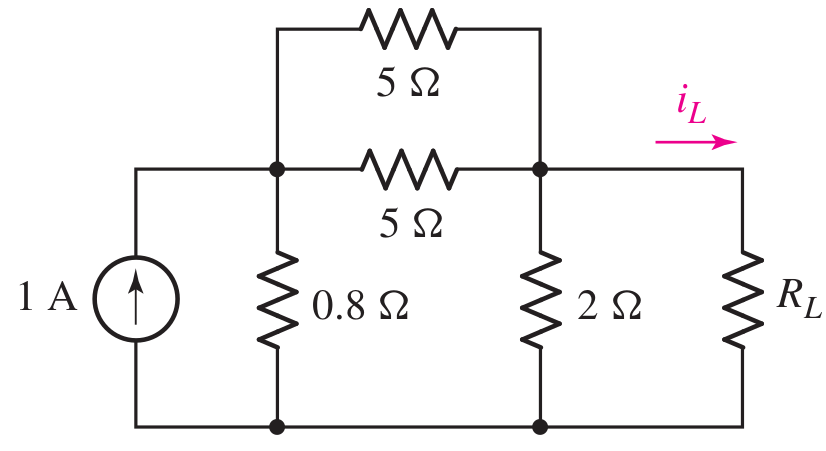
\includegraphics[scale=.3]{c1}
 \\
 
 2- Utilice el teorema de Thévenin para obtener un equivalente sencillo de dos componentes del circuito que se muestra en la figura.
 
 b) Use su circuito equivalente para determinar la potencia suministrada a una resistencia de 100 $\Omega$ conectada en las terminales a circuito abierto.
 
 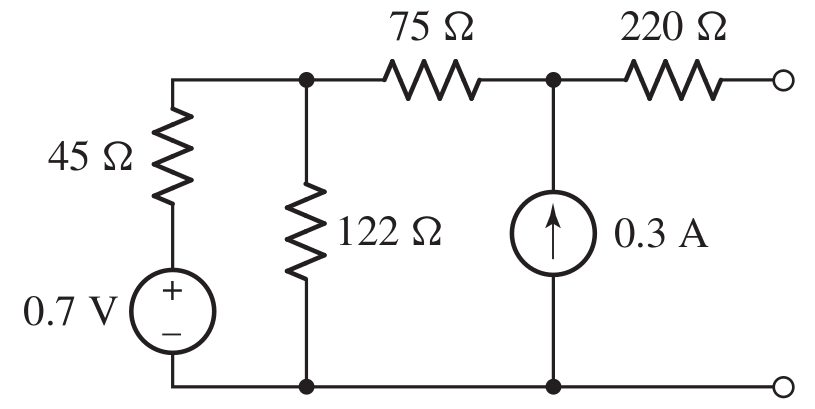
\includegraphics[scale=0.3]{c2}
 \\

  3- Determine los equivalente de Thévenin del circuito representado en la figura visto desde las terminales a circuito abierto.
 
 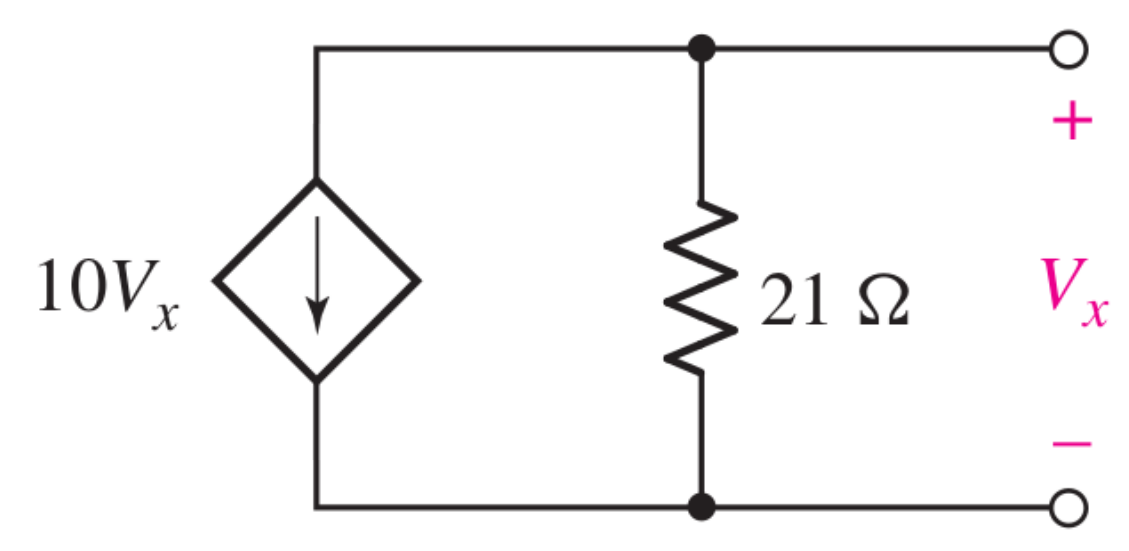
\includegraphics[scale=0.2]{c3_1}

 \pagebreak
  
 4- Determine el equivalente de Thévenin del circuito dibujado en la figura visto desde las terminales a y b.
 
  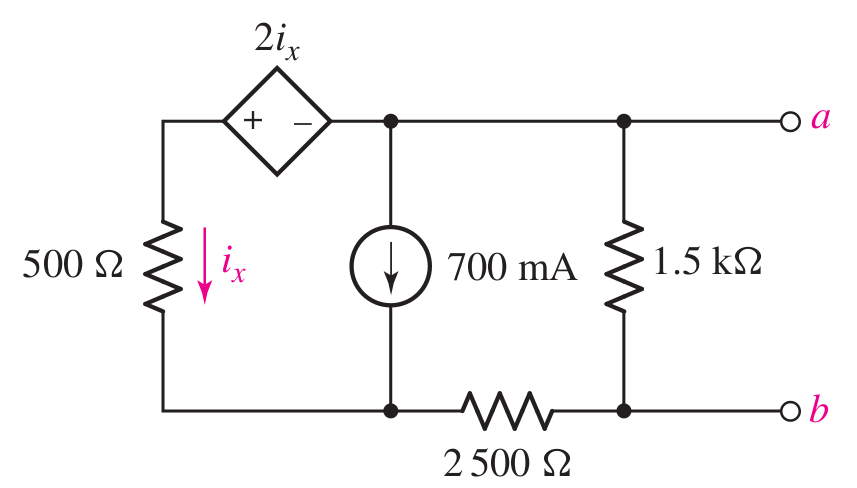
\includegraphics[scale=0.3]{c4}
  \\
  
 5- Determine la corriente marcada como $I$ en el circuito de la figura realizando primero la transformación de fuentes y las combinaciones paralelo-serie según se necesite para reducir el circuito tanto como sea posible.
 \\
 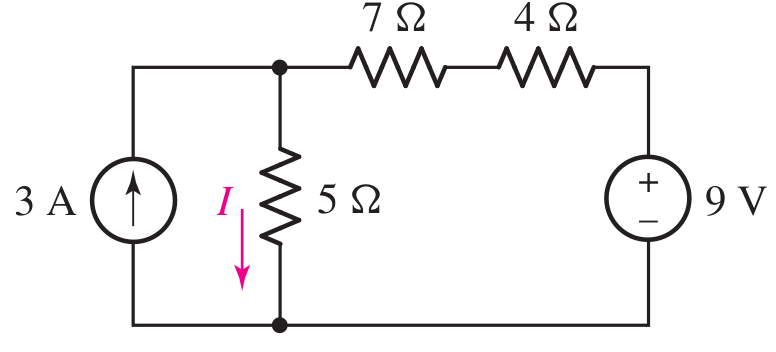
\includegraphics[scale=0.35]{c5}
 \\
 
 6- Usando superposición, determine la tensión marcada como $v_x$ en el circuito representado en la figura. 
 
 b) ¿A qué valor se debe cambiar la fuente de 2 A para reducir $v_x$ en 10\%?
 
  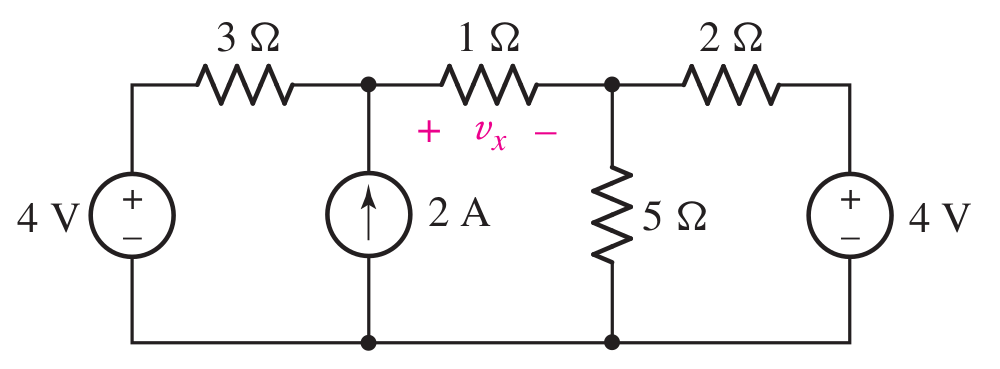
\includegraphics[scale=0.35]{c6}
 
\end{document}